\documentclass[main.tex]{subfiles}

\begin{document}

% \textcolor{red}{Вводная лекция}

\section{Лекция 02.04.2021 (Валов А.В.)}

\subsection{Модель Planar3D ILSA}

\subsubsection{Предположения модели}

Предположения модели:

1) одна трещина (плоская);

2) среда однородна по $E$ и $\nu$;

3) работаем в рамках линейно-упругой механики разрушения (ЛМР);

4) жидкость ньютоновская с вязкостью $\mu$;

5) утечки по Картеру, $C_L$;

6) среда однородна по $K_{Ic}$ и $C_L$;

7) пренебрегаем силой тяжести;

8) отсутствует fluid lag.

\subsubsection{Вспомогательные обозначения}

Перед тем, как переходить к уравнениям, давайте введём вспомогательные обозначения:
\beq
\mu'=12\mu,\,\,\,\,\,\,\,\,\,\,
E'=\frac{E}{1-\nu^2},\,\,\,\,\,\,\,\,\,\,
K'=4\left(\frac{2}{\pi}\right)^{1/2}K_{Ic},\,\,\,\,\,\,\,\,\,\,
C'=2C_L
\eeq
(мы просто на основе входных параметров модели ввели некоторые обозначения, которые позволят нам записать уравнения чуть-чуть короче).

\subsubsection{Основные уравнения}

Теперь давайте переходить к уравнениям. У нас есть две составляющие: упругая среда, которая описывается неким уравнением упругости, и течение жидкости по трещине.

\textbf{Упругость.}

Упругость связывает давление жидкости в трещине и раскрытие этой трещины:
\beq
p(x,y,t)=\sigma_h(y)-\frac{E'}{8\pi}\int\limits_{A(t)}\frac{w(x',y',t)dx'dy'}{\left[(x'-x)^2+(y'-y)^2\right]^{3/2}}
\eeq


\textbf{Гидродинамика.}

Уравнение для течения жидкости в трещине.
\beq\label{GeneralReynolds}
\frac{\partial w}{\partial t}+\text{div }{\vec{q}}=Q_0(t)\delta(x-x_0,y-y_0)-\frac{C'}{\sqrt{t-t_0(x,y)}},
\eeq
где $\vec{q}$ -- это поток жидкости по трещине; $Q_0(t)\delta(x-x_0,y-y_0)$ -- точечный источник потока; $t_0(x,y)$ -- это время, при котором фронт трещины находился в точке $(x,y)$; величина $(t-t_0)$ -- это время экспозиции (смысл времени экспозиции в том, что жидкость начинает утекать из некоторой точки только тогда, когда фронт трещины до неё доедет).

Для потока $\vec{q}$ выполняется закон Пуазейля:
\beq\label{q_poiseuille}
\vec{q}=-\frac{w^3}{\mu'}\nabla p
\eeq
(т.е. поток жидкости по трещине берём из аналитического решения уравнения Навье-Стокса для канала с фиксированной шириной $w$)


Подставляя \eqref{q_poiseuille} в \eqref{GeneralReynolds} , получаем уравнение Рейнольдса, которое описывает течение жидкости по трещине:
\beq
\frac{\partial w}{\partial t}-\text{div}{\left(\frac{w^3}{\mu'}\nabla p\right)}=Q_0(t)\delta(x-x_0,y-y_0)-\frac{C'}{\sqrt{t-t_0(x,y)}},
\eeq

\begin{center}
\includegraphics[width=.6\textwidth, page=3]{Valov_slides.pdf}
\end{center}

\subsubsection{Граничные условия}

Первое граничное условие следует из предположения, что мы работаем в рамках линейно-упругой механики разрушения:
\beq
\lim\limits_{s\to 0}\frac{w(s)}{s^{1/2}}=\frac{K'}{E'}
\eeq
(равносильно условию $K_{I}=K_{Ic}$)

Второе граничное условие -- это условие нулевого потока на кончике трещины:
\beq
\vec{q}\cdot\vec{n}\to 0\text{ при } s\to 0\,\,\,\Leftrightarrow\,\,\, \lim\limits_{s\to 0}{\frac{w^3}{\mu}\frac{\partial p}{\partial s}}=0
\eeq
(условие отсутствия fluid lag)
\\

\textbf{Универсальное асимптотическое решение в окрестности фронта трещины}

Сделаем небольшое лирическое отступление про линейные асимптотики.
Зачем нам линейные асимптотики?
У нас есть плоская трещина.
Локально если рассмотреть некую окрестность фронта, то задача очень похожа на распространение одномерной полубесконечной трещины с постоянной скоростью $v$.
У этой задачи есть три предельных режима.
Здесь наверное стоит начать с того, что в кончике трещины на самом деле есть 3 конкурирующих процесса.

Первый процесс (toughness) -- это  затрачивание энергии на образование новой поверхности трещины (т.е. чтобы образовать новую поверхность трещины, требуется выполнение критерия разрушения).

Второй процесс (leak-off) -- это утекание жидкости из трещины.

Третий процесс (viscosity) -- это вязкая диссипация жидкости по трещине (жидкость течёт с параболическим фронтом, есть трение, энергия затрачивается на то, чтобы протолкнуть эту жидкость по трещине).

\begin{center}
\includegraphics[width=.6\textwidth, page=4]{Valov_slides.pdf}
\end{center}

Если брать только один из этих эффектов, а двумя другими пренебрегать, то мы можем получить 3 предельных режима:
\begin{itemize}
	\item доминирование разрушения породы
	\beq
	w_k=\frac{K'}{E'}s^{1/2}
	\eeq
	\item доминирование утечек
	\beq
	w_{\tilde{m}}=\beta_{\tilde{m}}\left(\frac{4\mu'^2v\,C'^2}{E'^2}\right)^{1/8}s^{5/8}
	\eeq
	\item доминирование вязкости
	\beq
	w_m=\beta_m\left(\frac{\mu'v}{E'}\right)^{1/3}s^{2/3}
	\eeq
\end{itemize}

Для более точного моделирования было бы полезно учитывать не один из трёх режимов, а все 3 режима сразу (и переходные режимы между ними).

Всю задачу о полубесконечной трещине с учётом всех трёх эффектов можно приближённо решить и получить универсальное асимптотическое решение:
\beq
\frac{s^2v\mu'}{E'w^3}=g_\delta\left(\frac{K's^{1/2}}{E'w},\frac{2s^{1/2}C'}{w\,v^{1/2}}\right)
\eeq
(это приближённое решение, но оно в пределах одного процента или даже лучше совпадает с точным решением; исходная задача полубесконечной трещины представляет собой нелинейное интегральное уравнение на полубесконечной прямой, которое неизвестно, как решить несложными способами; однако получили, что приближённо решение задачи полубесконечной трещины можно свести к функциональной зависимости между $w$ и $s$).

Введя следующие обозначения
\beq
\hat{S}(w,s)=\frac{s^2v\mu'}{E'w^3}\,\,\,\,\,\,\,\,\,\,\hat{K}(w,s)=\frac{K's^{1/2}}{E'w}\,\,\,\,\,\,\,\,\,\,\hat{C}(w,s)=\frac{2s^{1/2}C'}{w\,v^{1/2}}
\eeq
перепишем универсальную асимптотику
\beq
\hat{S}(w,s)=g_\delta\left(\hat{K}(w,s),\hat{C}(w,s)\right)
\eeq


Функция $g_\delta$ -- это функция, у которой есть вполне определённый аналитический вид.
Т.е. теперь нет необходимости решать дифференциальное или интегральное уравнение.
Если мы знаем $s$, то можем его подставить и, решив нелинейное алгебраическое уравнение, найти $w$.
Т.е. зная расстояние до фронта трещины, мы можем найти раскрытие.
Или, зная раскрытие, можем найти расстояние до фронта трещины.
Другими словами, в полученной асимптотике всегда предполагается, что нам известна одна из величин: или расстояние до фронта, или раскрытие трещины.
И по одному из этих параметров находится другой параметр, например, с помощью метода Ньютона.

Полученная универсальная асимптотика верна только в случае $v>0$ (трещина куда-то постоянно едет, т.е. выполняется критерий разрушения $K_{I}=K_{Ic}$).
Если же трещина остановилась, то критерий разрушения не выполняется (т.е. $K_{I}<K_{Ic}$) и вместо универсальной асимптотики рассматривают toughness асимптотику:
\beq
w=\frac{K_{I}'}{\mu'}s^{1/2}
\eeq
(методы расчёта коэффициента $K_{I}'$ -- это отдельная кухня).

Таким образом, важно понимать, что универсальная асимптотика верна только для случая, когда выполнен критерий разрушения.


Зачем вспомнили при универсальную асимптотику?
Если мы локально рассмотрим кусочек трещины вблизи фронта, то там трещина движется одномерно с постоянной скоростью, а для этого случая у нас есть приближённое решение, которое близко к точному.

Вблизи кончика трещины самые большие градиенты, т.е. если мы разрабатываем численный метод для решения задачи, то особое внимание необходимо уделить кончику трещины, потому что там самые большие градиенты, а значит самые большие ошибки.

Идея заключается в следующем: хотим в окрестности кончика трещины найти аналитическое решение (оно у нас есть) и сказать, что в окрестности фронта трещины раскрытие должно равняться некоторому аналитическому раскрытию.


Т.е. условно мы в кончике трещины задачу решаем практически точно, а когда мы отдаляемся от кончика трещины, то там градиенты искомых функций меньше и ошибка численного алгоритма будет меньше.

Мы пытаемся с помощью универсальной асимптотики практически точно решить задачу в окрестности фронта, тем самым уменьшив численную ошибку будущего алгоритма.

При этом эта универсальная асимптотика покрывает условие $K_{I}=K_{Ic}$, которое было изначально (т.е. мы не теряем это условие).
\\

Итак, мы выписали уравнения, граничные условия, вспомнили асимптотики и решили использовать универсальную асимптотику в окрестности фронта в качестве точного решения, т.е. первое граничное условие перепишем в виде:
\beq
w(s)\sim w_a(s)\text{ при }s\to 0
\eeq

\subsubsection{Дискретизация области моделирования. Классификация элементов}

В принципе мы всё обсудили для того, чтобы начать разрабатывать численный алгоритм.
Давайте к нему и перейдём.
Для того, чтобы записать численный алгоритм, сначала нужно разобраться с областью моделирования.

\begin{center}
\includegraphics[width=.6\textwidth, page=5]{Valov_slides.pdf}
\end{center}

Есть плоскость, которую мы покрываем прямоугольными элементами (с шириной $dx$ и с высотой $dy$).
Есть фронт трещины, который распространяется со скоростью $v$, и эта скорость локально в каждом участке фронта различная (каждый участок фронта едет со своей скоростью).
Рассматриваемая трещина покрывает собой некоторый набор прямоугольных элементов.
Эти элементы удобно будет разделить на 3 категории:

1) концевые элементы (пересекаются контуром трещины и частично заполнены жидкостью);

2) внутренние элементы (находятся внутри трещины и полностью заполнены жидкостью);

3) опорные элементы (тоже являются внутренними элементами, но дополнительно граничат с концевыми элементами).

\subsubsection{Дискретизация уравнений}

Итак, есть плоскость с сеткой, теперь необходимо заняться дискретизацией искомых функций.
У нас две искомые функции:

1) раскрытие трещины $w(x,y,t)$, которое мы будем аппроксимировать кусочно-постоянно, т.е.
\beq
w(x,y,t)=\sum_{m,n}w_{m,n}(t)H_{m,n}(x,y),
\eeq
где
\beq
H_{i,j}(x,y)=
\begin{cases}
1,\,\,\,(x,y)\in A_{i,j}\\
0,\,\,\,(x,y)\notin A_{i,j}	
\end{cases}
\eeq

2) давление $p(x,y,t)$, которое аналогично будем аппроксимировать кусочно-постоянно.
\\

\textbf{Дискретизация уравнения упругости}

Подставляя кусочно-постоянную аппроксимацию раскрытия $w$ в уравнение упругости, получаем:
\beq
p_{i,j}(t)=\sigma_{h_{i,j}}+\sum\limits_{k,l}C_{i,j,k,l}w_{k,l}(t),
\eeq
где
\beq
C_{i,j,k,l}=-\frac{E'}{8\pi}\left[\frac{\sqrt{(x_i-x)^2+(y_j-y)^2}}{(x_i-x)(y_j-y)}\right]_{x=x_k-\frac{\Delta x}{2},\,y=y_l-\frac{\Delta y}{2}}^{x=x_k+\frac{\Delta x}{2},\,y=y_l+\frac{\Delta y}{2}}
\eeq

Здесь использовали обозначение квадратных скобок с индексами:
\beq
\left[f\right]_{x=x_1,\,y=y_1}^{x=x_2,\,y=y_2}=f(x_1,y_1)+f(x_2,y_2)-f(x_1,y_2)-f(x_2,y_1)
\eeq

$C_{i,j,k,l}$ -- это матрица упругости (характеризует упругое влияние элемента с индексами $(k,l)$ на элемент с индексами $(i,j)$).

Заметим, что матрица упругости зависит только от входных параметров (от свойств пласта) и выбранной сетки, т.е. эту матрицу требуется посчитать только один раз (нет необходимости пересчитывать её в процессе расчёта).
\\

\textbf{Дискретизация уравнения Рейнольдса}

Далее обсудим более сложную часть, а именно дискретизацию уравнений Рейнольдса.
Поскольку уравнение Рейнольдса изначально появилось из закона сохранения массы, то нам нужно его аппроксимировать таким образом, чтобы масса сохранялась (т.е. нам нужна консервативная численная схема интегрирования).

Постепенно будем выводить консервативную схему.

Уравнение Рейнольдса:
\beq
\frac{\partial w}{\partial t}-\text{div}{\left(\frac{w^3}{\mu'}\nabla p\right)}=Q_0(t)\delta(x-x_0,y-y_0)-\frac{C'}{\sqrt{t-t_0(x,y)}},
\eeq

Проинтегрируем уравнение Рейнольдса от $t-\Delta t$ до $t$ (т.е. возьмём 1 шаг по времени и по этому шагу по времени просто проинтегрируем уравнение):
\beq
\underbrace{\int\limits_{t-\Delta t}^{t}{\frac{\partial w}{\partial \tau}}d\tau}_{\text{интегрируем точно}}-\underbrace{\int\limits_{t-\Delta t}^{t}{\text{div}{\left(\frac{w^3}{\mu'}\nabla p\right)}d\tau}}_{\substack{\text{интегрируем приближённо}\\\text{по формуле правых}\\\text{прямоугольников}}}=\underbrace{\int\limits_{t-\Delta t}^{t}{\varphi(\tau)d\tau}}_{\text{не трогаем}},
\eeq
где
\beq
\varphi(t)=Q_0(t)\delta(x-x_0,y-y_0)-\frac{C'}{\sqrt{t-t_0(x,y)}}
\eeq

Для интегрирования дивергенции используем именно формулу правых прямоугольников (а, например, не формулу Симпсона), чтобы итоговая численная схема была проще.
При использовании формулы Симпсона не факт, что схема будет устойчива.

Воспользовавшись формулой Ньютона-Лейбница и формулой правых прямоугольников, получаем:
\beq
w(t)-w(t-\Delta t)-\Delta t\left[\text{div}{\left(\frac{w^3}{\mu'}\nabla p\right)}\right]_t=\int\limits_{t-\Delta t}^{t}{\varphi(\tau)d\tau}
\eeq


\end{document}